\section{Improvement Strategies}
\subsection{Hyperparameter Tuning}
We explored three diverse strategies to improve our initial speech command detection system: hyperparameter tuning, ensembling, and data augmentation. Each strategy aims to enhance detection accuracy and reduce associated costs.
\subsubsection{Description}
We tuned the hyperparameters of our classifier, to enhance the detection accuracy and reduce the associated costs. We identified the following key steps for our classifier:
\begin{itemize}
  \item \textbf{Adaptive Learning Rate:} Adjusted by epoch schedule to control the step size during gradient descent.
  \item \textbf{Architecture:} Varied the depth and width of the neural network as well as the base paradigm to find an optimal architecture.
  \item \textbf{Anti-Overfitting:} Applied dropout, early stopping, ADAM to prevent overfitting.
\end{itemize}


\subsubsection{Outcome}
The tuning process was conducted using grid search on the validation set.
The optimized hyperparameters finally led to a smooth training process with promising validation as shown in figures
\ref{fig:tuned_learning_curves} and \ref{fig:tuned_heatmap}.

%\begin{figure}[h]
%\centering
%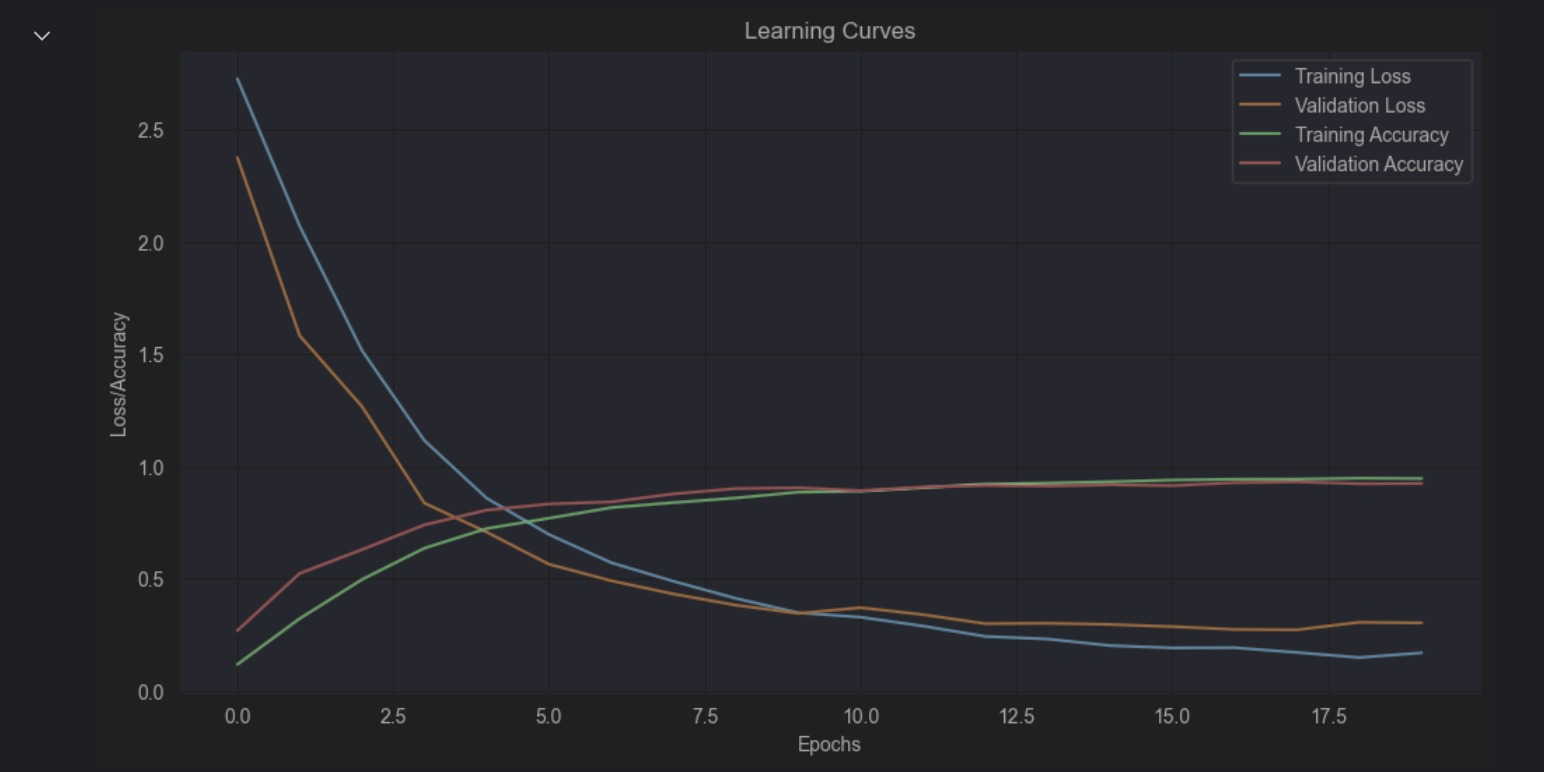
\includegraphics[width=0.6\textwidth]{fig/tuned_learning_curves}
%\caption{Impact of hyperparameter tuning on training and validation.}
%\label{fig:hyperparameter_tuning}
%\end{figure}

\begin{figure}[!ht]
	\centering
	\begin{minipage}{0.49\textwidth}
		\centering
		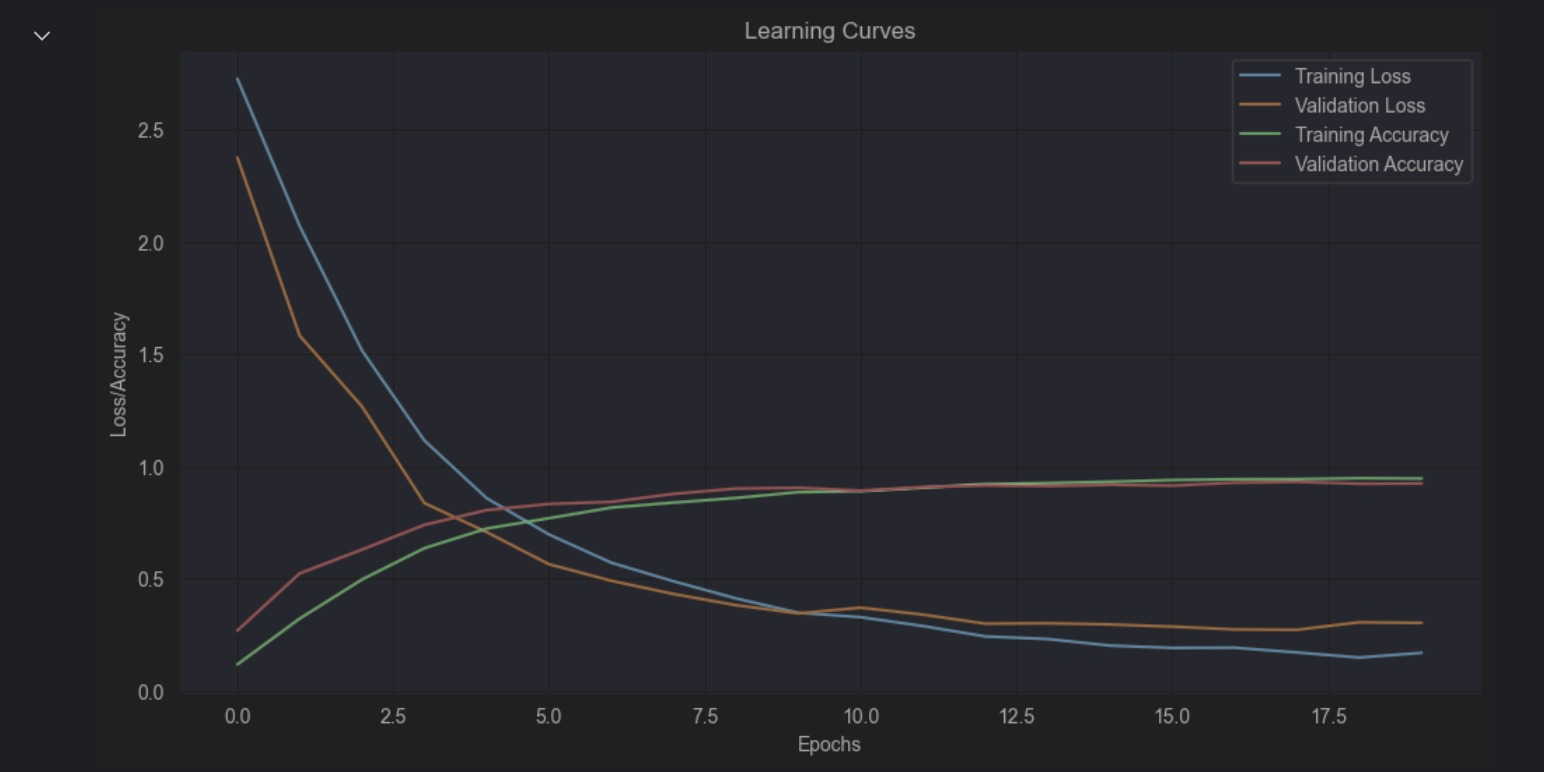
\includegraphics[scale=0.15]{fig/tuned_learning_curves}
		\caption{Learning Curve After Tuning.}
      \label{fig:tuned_learning_curves}
	\end{minipage}\hfill
	\begin{minipage}{0.2\textwidth}
		\centering
		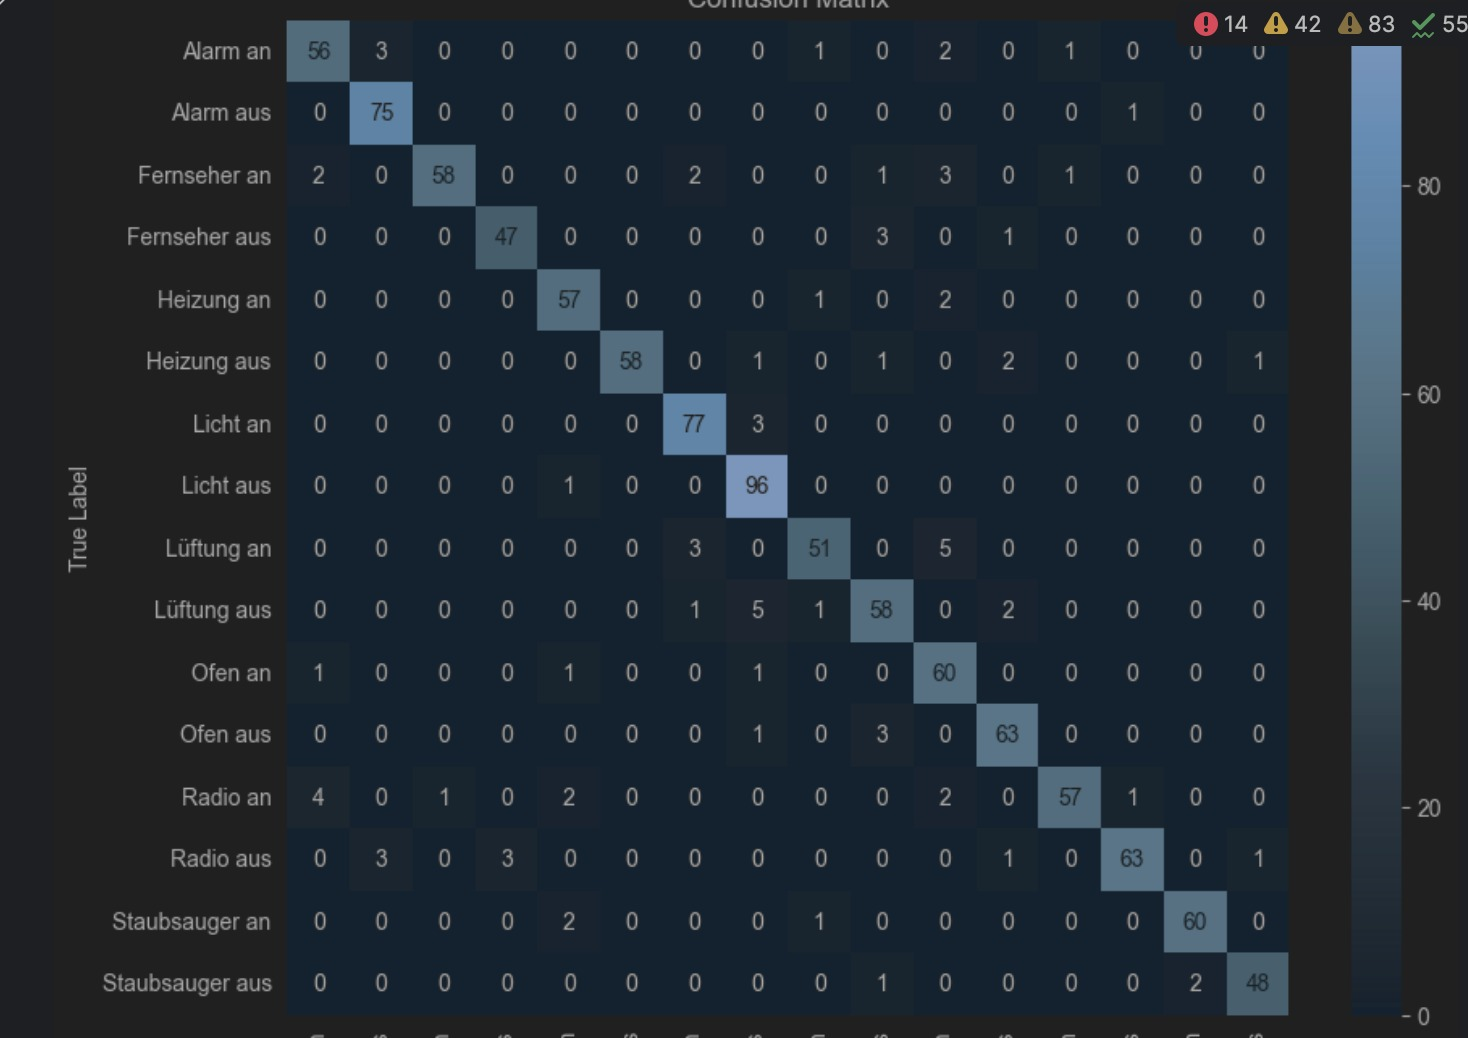
\includegraphics[scale=0.1]{fig/tuned_heatmap}
		\caption{Heatmap After Tuning.}
        \label{fig:tuned_heatmap}
	\end{minipage}

\end{figure}

\subsection{Ensembling}
\subsubsection{Description}
We used ensembling to combine the predictions from multiple models to leverage their individual strengths and enhance overall robustness. Our approaches here were:
\begin{itemize}
  \item \textbf{Boosting:} Sequentially trained classifiers, where each classifier attempts to correct the errors of its predecessor.
  \item \textbf{Bagging:} Combined predictions from multiple instances of the same classifier trained on different subsets of the training data.
\end{itemize}

\subsubsection{Outcome}
The ensemble model was evaluated on the validation set and reduced the number of false positives and overall costs, as depicted in Table \ref{tab:ensemble_results}.

\begin{table}[h]
\centering
\begin{tabular}{lccc}
\toprule
Metric & Single Model & Ensemble Model \\
\midrule
True Positives & 70 & 75 \\
False Negatives & 5 & 4 \\
False Positives & 15 & 10 \\
Cross-Triggers & 8 & 5 \\
Total Cost & -10 & -20 \\
\bottomrule
\end{tabular}
\caption{Evaluation results comparing a single model and the ensemble model.}
\label{tab:ensemble_results}
\end{table}

\subsection{Data Augmentation}
\subsubsection{Description}
We augmented the training data with various transformations, including noise addition, pitch changes, and speed variations.
These techniques helped the model generalize better to unseen data, particularly noisy recordings
(h)owever, traditional models still struggled in real-world scenarios).

\subsubsection{Outcome}
Augmenting the training data resulted in a model that was more robust to variations in the audio environment,
leading to improved detection performance in noisy conditions.
\ref{fig:data_augmentation}.

\begin{figure}[h]
\centering
\includegraphics[width=0.6\textwidth]{fig/data_augmentation.png}
\caption{Impact of data augmentation on detection performance and costs.}
\label{fig:data_augmentation}
\end{figure}
